\chapter{Distance in Graphs}

\section{introduction}

We have a natural understanding of the ``distance'' between two objects in our physical space. But there are many other ways of defining distances. E.g., the distance between people could be the positive difference of their birth years or the number of acquaintances you need to connect one to the other.

In this chapter we will introduce a notion of distance of vertices in a graph. But first let us note what are the characterising properties that make us call all these concepts ``distances''.

% 2.1 Definition
\begin{definition}
Let $X$ be any set. We call a function $d: X \times X \to \mathbb{R}^{\ge 0} \cup \{\infty\}$ a \textbf{\color{red}metric} if it satisfies for all $x,y,z \in X$:
\begin{enumerate}
    \item[1)] $d(x,y) \ge 0$
    \item[2)] $d(x,y) = 0$ iff $x=y$
    \item[3)] $d(x,y) = d(y,x)$
    \item[4)] $d(x,z) \le d(x,y) + d(y,z)$ (\textbf{\color{red}Triangle Inequality})
\end{enumerate}
We then call the pair $(X,d)$ a \textbf{\color{red}metric space}.
\begin{center}
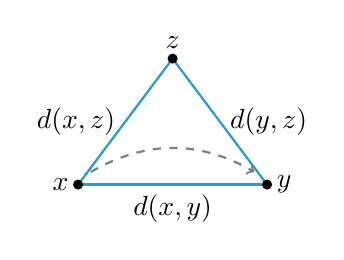
\begin{tikzpicture}[scale=0.8]
    \coordinate (x) at (0,0);
    \coordinate (y) at (3,0);
    \coordinate (z) at (1.5, 2);
    
    \draw[cyan!80!black, thick] (x) -- (y) node[midway, below, black] {$d(x,y)$};
    \draw[cyan!80!black, thick] (x) -- (z) node[midway, left, black] {$d(x,z)$};
    \draw[cyan!80!black, thick] (z) -- (y) node[midway, right, black] {$d(y,z)$};
    
    \filldraw (x) circle (2pt) node[left] {$x$};
    \filldraw (y) circle (2pt) node[right] {$y$};
    \filldraw (z) circle (2pt) node[above] {$z$};
    
    % Visualizing triangle inequality shortcut
    \draw[->, gray, dashed, thick] (0.2, 0.2) to[bend left] (2.8, 0.2);
\end{tikzpicture}
\end{center}
\end{definition}

% 2.2 Example
\begin{example}
Consider $X=\mathbb{R}$ and $d: \mathbb{R} \times \mathbb{R} \to \mathbb{R}^{\ge 0}$ via $d(x,y) := |x-y|$. Then $(\mathbb{R}, d)$ is a metric space.
\end{example}

Now we are ready to define a metric on an arbitrary graph.

% 2.3 Definition
\begin{definition}
Let $G$ be any graph and $u,v \in V_G$. We define the \textbf{\color{red}distance $d(u,v)$} between $u$ and $v$ as the length of the shortest $uv$-path in $G$, i.e.
\[ d(u,v) := \min \{ \text{length}(P) \mid P \text{ is a } uv\text{-path} \}. \]
If there is no such path, we set \textbf{\color{red}$d(u,v) := \infty$}.

2) If $d(u,v)=k$, then any $uv$-path of length $k$ is called a \textbf{\color{red}geodesic}.
\end{definition}

% 2.4 Remark
\begin{remark}
\begin{enumerate}
    \item[1)] We may write $d_G(u,v)$ to emphasize that we consider the distance in $G$.
    \item[2)] While in $(\mathbb{R}, d)$ geodesics are unique, in general this is not the case. Consider for example two opposite poles on a sphere.
    \item[3)] $d(x,y)=\infty$ iff $x$ and $y$ are in different connected components.
    \item[4)] $(V_G, d)$ is a metric space for any connected graph $G$.
\end{enumerate}
\end{remark}

We call something eccentric if it is away from the usual. Similarly, in graphs we measure by eccentricity how far a vertex is from the center. Consider the following notions on a cycle:

\begin{center}
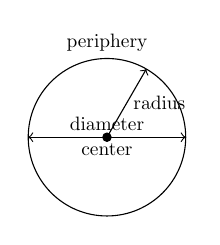
\begin{tikzpicture}
    \draw (0,0) circle (1cm);
    \filldraw (0,0) circle (1.5pt) node[below, scale=0.7] {center};
    \draw[->] (0,0) -- (60:1) node[midway, right, scale=0.7] {radius};
    \draw[<->] (-1,0) -- (1,0) node[midway, above, scale=0.7] {diameter};
    \node[scale=0.7] at (0, 1.2) {periphery};
\end{tikzpicture}
\end{center}

% 2.5 Definition
\begin{definition}
\begin{enumerate}
    \item[1)] The \textbf{\color{red}eccentricity $ecc(v)$} of a vertex $v$ is its greatest distance to any other vertex, i.e. $ecc(v) = \max \{ d(u,v) \mid u \in V_G \}$.
    \item[2)] The \textbf{\color{red}radius $rad(G)$} is the smallest possible eccentricity and the \textbf{\color{red}diameter $diam(G)$} is the largest possible eccentricity.
    \item[3)] The \textbf{\color{red}center $C(G)$} is the set $\{v \in V_G \mid ecc(v) = rad(G)\}$ and the \textbf{\color{red}periphery $P(G)$} is the set $\{v \in V_G \mid ecc(v) = diam(G)\}$.
\end{enumerate}
\end{definition}

% 2.6 Example
\begin{example}
1) Consider $P_5$, the path of length 4, i.e.
\begin{center}
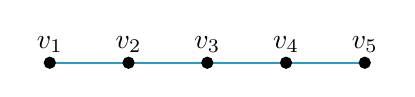
\begin{tikzpicture}
    \draw[cyan!80!black, thick] (0,0) -- (4,0);
    \foreach \i in {1,...,5} \filldraw (\i-1, 0) circle (2pt) node[above] {$v_\i$};
\end{tikzpicture}
\end{center}
Then
\begin{align*}
    d(v_1, v_i) &= i-1, \text{ whence } ecc(v_1) = \max\{0,1,2,3,4\} = 4. \\
    d(v_2, v_i) &= |i-2|, \text{ whence } ecc(v_2) = \max\{1,0,1,2,3\} = 3. \\
    d(v_3, v_i) &= |i-3|, \text{ whence } ecc(v_3) = \max\{2,1,0,1,2\} = 2. \\
    d(v_4, v_i) &= |i-4|, \text{ whence } ecc(v_4) = \max\{3,2,1,0,1\} = 3. \\
    d(v_5, v_i) &= |i-5|, \text{ whence } ecc(v_5) = \max\{4,3,2,1,0\} = 4.
\end{align*}
Hence $rad(P_5) = \min\{ecc(v) \mid v \in V\} = \min\{4,3,2,3,4\} = 2$.
Also $C(P_5) = \{v \in V \mid ecc(v) = rad(P_5)\} = \{v_3\}$.
Further $diam(P_5) = \max\{ecc(v) \mid v \in V\} = \max\{4,3,2,3,4\} = 4$.
And $P(P_5) = \{v \in V \mid ecc(v) = diam(P_5)\} = \{v_1, v_5\}$.

2) Consider $G := C_6$, the cycle of length 6, i.e. $G=$
\begin{center}
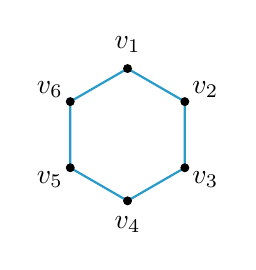
\begin{tikzpicture}[scale=0.7, baseline=(current bounding box.center)]
    \foreach \i in {1,...,6} \coordinate (v\i) at (90+60-60*\i : 1.2);
    \draw[cyan!80!black, thick] (v1)--(v2)--(v3)--(v4)--(v5)--(v6)--(v1);
    \foreach \i in {1,...,6} \filldraw (v\i) circle (2pt) node[anchor=center, shift={(90+60-60*\i:0.3)}] {$v_\i$};
\end{tikzpicture}
\end{center}
Then $d(v_0, v_i)$... (calculations symmetric).
$ecc(v_0) = \max\{0,1,2,3,2,1\} = 3$.
Actually $ecc(v) = 3$ for all $v$.
Hence, $rad(G) = \min\{3,3,3,3,3,3\} = 3$.
Whence $C(G) = V_G$.
Further, $diam(G) = \max\{3,3,3,3,3,3\} = 3$.
And $P(G) = V_G$.
\end{example}

\topic{Intermezzo}

I: Find $rad(G), diam(G), C(G)$ and $P(G)$ of the following:
1) $G_1 = P_{10}$ \hspace{1cm} 2) $G_2 = K_6$

II: Consider
\begin{center}
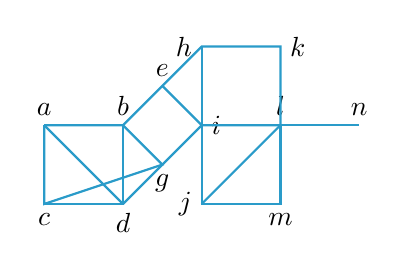
\begin{tikzpicture}
    % Graph from Intermezzo
    \coordinate (a) at (0,1); \node[above] at (a) {$a$};
    \coordinate (b) at (1,1); \node[above] at (b) {$b$};
    \coordinate (e) at (1.5, 1.5); \node[above] at (e) {$e$};
    \coordinate (h) at (2, 2); \node[left] at (h) {$h$};
    \coordinate (k) at (3, 2); \node[right] at (k) {$k$};
    \coordinate (i) at (2, 1); \node[right] at (i) {$i$};
    \coordinate (l) at (3, 1); \node[above] at (l) {$l$};
    \coordinate (n) at (4, 1); \node[above] at (n) {$n$};
    \coordinate (f) at (1.5, 0.5); \node[below] at (f) {$g$}; % Wait, note says g below f
    \coordinate (c) at (0,0); \node[below] at (c) {$c$};
    \coordinate (d) at (1,0); \node[below] at (d) {$d$};
    \coordinate (j) at (2,0); \node[left] at (j) {$j$};
    \coordinate (m) at (3,0); \node[below] at (m) {$m$};
    
    % Draw left square
    \draw[cyan!80!black, thick] (a)--(b)--(f)--(c)--(a); 
    \draw[cyan!80!black, thick] (c)--(d)--(b); % Cross in square
    \draw[cyan!80!black, thick] (a)--(d); % Cross
    \draw[cyan!80!black, thick] (f)--(d);
    
    % Connection to right part
    \draw[cyan!80!black, thick] (b)--(e)--(h)--(k)--(l)--(i)--(e);
    \draw[cyan!80!black, thick] (h)--(i); % vertical? No
    \draw[cyan!80!black, thick] (f)--(i);
    \draw[cyan!80!black, thick] (i)--(j)--(m)--(l)--(n);
    \draw[cyan!80!black, thick] (j)--(l);
    
    % Let's approximate the sketch better based on standard Intermezzo style
    % It looks like two house/square shapes connected.
    % I will draw a representative graph based on the nodes shown.
\end{tikzpicture}
\end{center}
Find:
\begin{itemize}
    \item $d(b,c), d(h,k), d(a,m)$
    \item $ecc(v)$ for all $v \in V_G$
    \item $rad(G), diam(G), C(G), P(G)$.
\end{itemize}

% 2.7 Lemma
\begin{lemma}
For any graph $G$ we have $rad(G) \le diam(G) \le 2 rad(G)$.
\end{lemma}

\begin{proof}
We have $rad(G) \le diam(G)$ by definition. For the other inequality, pick $v \in C(G)$ arbitrary and consider $u,w \in V_G$ arbitrary s.t. $d(u,w) = diam(G)$. Then
\[ d(u,w) \le d(u,v) + d(v,w) \le ecc(v) + ecc(v) = 2 rad(G). \qedhere \]
\end{proof}

% 2.8 Theorem
\begin{theorem}
Every graph $G$ is isomorphic to the graph induced by the center of another graph $H$, i.e. ex. $H$ s.t. $G \cong \langle C(H) \rangle$.
\end{theorem}

\begin{proof}
Let $G$ be arbitrary. We build a new graph $H$ which contains $G$ as an induced subgraph via: $V_H = V_G \cup \{u,x,y,z\}$, i.e. adding 4 new vertices to $G$. Further, let $E_H = E_G \cup \{ux, yz\} \cup \{xv, vy \mid v \in V_G\}$.

\begin{center}
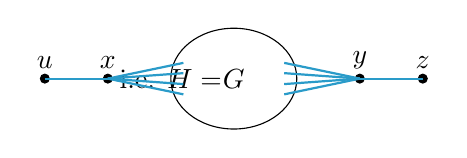
\begin{tikzpicture}[scale=0.8]
    \node at (-1,0) {i.e. $H=$};
    \draw (0,0) ellipse (1cm and 0.8cm); \node at (0,0) {$G$};
    
    \coordinate (x) at (-2,0); \filldraw (x) circle (2pt) node[above] {$x$};
    \coordinate (y) at (2,0); \filldraw (y) circle (2pt) node[above] {$y$};
    \coordinate (u) at (-3,0); \filldraw (u) circle (2pt) node[above] {$u$};
    \coordinate (z) at (3,0); \filldraw (z) circle (2pt) node[above] {$z$};
    
    \draw[cyan!80!black, thick] (u)--(x);
    \draw[cyan!80!black, thick] (y)--(z);
    
    % Connections to G
    \foreach \ang in {150, 170, 190, 210} \draw[cyan!80!black, thick] (x) -- (-0.8, {0.5*sin(\ang)});
    \foreach \ang in {-30, -10, 10, 30} \draw[cyan!80!black, thick] (y) -- (0.8, {0.5*sin(\ang)});
\end{tikzpicture}
\end{center}

Now $ecc(v)=2$ for any $v \in V_G$. Nevertheless, $d(u,z)=4$ and $d(x,z)=d(y,u)=3$, whence $ecc(w)>2$ for all $w \in V_H \setminus V_G$. Thus, $rad(H)=2$ and $C(H)=V_G$, whence $\langle C(H) \rangle \cong G$.
\end{proof}

% 2.9 Lemma
\begin{lemma}
A graph $G$ is isomorphic to the graph induced by the periphery of another graph $H$ iff either every vertex has eccentricity 1 or no vertex does.
\end{lemma}

\begin{proof}
``$\Rightarrow$'' We use proof by contraposition. Assume ex. $u \in V_G$ s.t. $ecc(u)=1 < diam(G)$. In particular, $G \ne P(G)$. Now, aiming for a contradiction, assume ex. $H$ s.t. $G \le H$ and $P(H) = V_G$.
As $G \ne P(G)$, we know that $H \ne G$ and $diam(H) \ge 2$. As $u \in V_G = P(H)$, there is some $w \in V_H$ s.t. $d(u,w)=diam(H)$. But then, $w \in P(H) \cong V_G$, and as $ecc(u)=1$, we also get $d(u,w)=1 < diam(H)$. Hence, $P(H)$ cannot be $V_G$.

``$\Leftarrow$'' If all vertices in $G$ have eccentricity 1 or 0, then $G$ is complete and $G \cong P(G)$. For the second case, assume $rad(G)>1$. And consider $H$ s.t. $V_H = V_G \cup \{v\}$ contains one new vertex which is connected to everyone else, i.e. $E_H = E_G \cup \{vx \mid x \in V_G\}$. Then, as $ecc(x) \ge 2$ for all $x \in V_G$,
\[ ecc_H(x) = \begin{cases} 2 & \text{if } x \in V_G \\ 1 & \text{if } x=v \end{cases}. \]
Hence, $diam(H)=2$ and $\langle P(H) \rangle = G$, as desired.
\end{proof}

\section{Adjacency Matrices}

We saw the visual benefits of studying graphs by their diagram. This is very useful to illustrate ideas and study small graphs. In applications on the other hand, when studying e.g. correlations of weather phenomena or social links, graphs tend to have thousands of vertices. Here, it is no longer practical to use neither the set- nor the diagram representation of graphs. The way computers store and analyze graphs is by using adjacency matrices.

% 2.10 Definition
\begin{definition}
Let $G$ be a graph of order $n$ with vertices $V_G = \{v_1, v_2, \dots, v_n\}$. The \textbf{\color{red}adjacency matrix} of $G$ is the matrix $A_G = (a_{ij}) \in M_{n \times n}$ defined via
\[ a_{ij} = \begin{cases} 1 & \text{if } v_i v_j \in E \\ 0 & \text{otherwise}. \end{cases} \]
We also write $A(i,j)$ for $a_{ij}$.
\end{definition}

% 2.11 Example
\begin{example}
Consider $G$ given by
\begin{center}
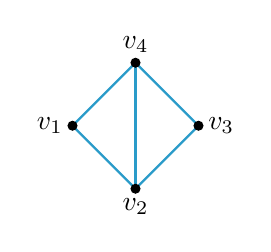
\begin{tikzpicture}[scale=0.8]
    \coordinate (v1) at (-1, 0); \node[left] at (v1) {$v_1$};
    \coordinate (v2) at (0, -1); \node[below] at (v2) {$v_2$};
    \coordinate (v3) at (1, 0); \node[right] at (v3) {$v_3$};
    \coordinate (v4) at (0, 1); \node[above] at (v4) {$v_4$};
    
    \draw[cyan!80!black, thick] (v1)--(v2)--(v3)--(v4)--(v1);
    \draw[cyan!80!black, thick] (v2)--(v4); % Cross
    
    \foreach \p in {v1,v2,v3,v4} \filldraw (\p) circle (2pt);
\end{tikzpicture}
\end{center}
Then $A_G \in M_{4 \times 4}$
\[ A_G = \begin{pmatrix} 0 & 1 & 0 & 1 \\ 1 & 0 & 1 & 1 \\ 0 & 1 & 0 & 1 \\ 1 & 1 & 1 & 0 \end{pmatrix} \]
is the adjacency matrix of $G$.
\end{example}

% 2.12 Remark
\begin{remark}
If $A_G = (a_{ij})$ is an adjacency matrix of a graph $G$, then
\begin{enumerate}
    \item[1)] $a_{ii} = 0$ for all $1 \le i \le |G|$
    \item[2)] $A$ is symmetric.
    \item[3)] $\sum_{j=1}^{|G|} a_{ij} = \deg(v_i)$ and thus $\sum_{i,j=1}^{|G|} a_{ij} = \sum_{i=1}^{|G|} \deg(v_i) = 2|E|$.
    \item[4)] $A_G$ is only unique up to reordering the vertices.
\end{enumerate}
\end{remark}

% 2.13 Example
\begin{example}
Let revisit the graph $G$ from 2.11. The fact that $A_G(2,3) \ne 0$ means that $v_2$ and $v_3$ are adjacent. And $A(1,3)=0$ says that $v_1$ and $v_3$ are not. Now consider
\[ A_G^2 = \begin{pmatrix} 0 & 1 & 0 & 1 \\ 1 & 0 & 1 & 1 \\ 0 & 1 & 0 & 1 \\ 1 & 1 & 1 & 0 \end{pmatrix} \begin{pmatrix} 0 & 1 & 0 & 1 \\ 1 & 0 & 1 & 1 \\ 0 & 1 & 0 & 1 \\ 1 & 1 & 1 & 0 \end{pmatrix} = \begin{pmatrix} 2 & 1 & 2 & 1 \\ 1 & 3 & 1 & 2 \\ 2 & 1 & 2 & 1 \\ 1 & 2 & 1 & 3 \end{pmatrix}. \]
Let's interpret the values of $A_G^2$.
Now, $A_G^2(1,3) = 2$. How did we compute it?
$A_G^2(1,3) = \sum_{j=1}^4 a_{1j} a_{j3}$. Now $a_{1j}a_{j3} = 1$ iff $v_1v_j$ and $v_j v_3$ are edges iff $(v_1, v_j, v_3)$ is a walk of length 2 from $v_1$ to $v_3$.
Hence, $A_G^2(1,3) = \sum a_{1j}a_{j3}$ is the number of walks from $v_1$ to $v_3$ of length 2. This generalises and provides a strong tool to study graphs.
\end{example}

% 2.14 Theorem
\begin{theorem}
Let $G$ be a graph with $V_G = \{v_1, \dots, v_n\}$ and $A_G$ the corresponding adjacency matrix. Then the entry $A_G^k(i,j)$ is the number of possible walks from $v_i$ to $v_j$ of length $k$.
\end{theorem}

\begin{proof}
We proceed by induction on the power $k$. (Note that $k=0$ works too).
\underline{$k=1$}: We get that $A(i,j) = \begin{cases} 0 & \text{iff } v_iv_j \notin E_G \text{ iff there are 0 } v_iv_j\text{-walks of length 1} \\ 1 & \text{iff } v_iv_j \in E_G \text{ iff there is 1 } v_iv_j\text{-walk of length 1} \end{cases}$.

\underline{$k \to k+1$}: Assume that $A^k(i,j)$ gives exactly the number of $v_iv_j$-walks of length exactly $k$. Let's denote $A^k = (b_{ij})$ and $A = (a_{ij})$.
Note that there is a $v_iv_j$-walk of length $k+1$ iff there ex. a vertex $v_\ell$ s.t. there is a $v_iv_\ell$-walk of length $k$ and an $v_\ell v_j$-walk of length one. Hence
\begin{align*}
    |\{v_iv_j\text{-walk of length } k+1\}| &= \sum_{\ell \mid v_\ell \in N(v_j)} |\{v_iv_\ell\text{-walk of length } k\}| \\
    &\overset{\text{I.H.}}{=} \sum_{\ell \mid v_\ell \in N(v_j)} b_{i\ell} = \sum_{\ell=1}^n b_{i\ell} a_{\ell j} \\
    &= \sum_{\ell=1}^n A^k(i,\ell) \cdot A(\ell, j) = A^{k+1}(i,j).
\end{align*}
\end{proof}

% 2.15 Corollary
\begin{corollary}
Let $G$ be a graph with $V_G=\{v_1, \dots, v_n\}$ and $A_G$ the adjacency matrix. Then $d(v_i, v_j) = \min \{ k \mid A^k(i,j) \ne 0 \}$.
(Recall that $A_G^0 = I_n$).
\end{corollary}

% 2.16 Definition
\begin{definition}
Let $G$ be a graph with adjacency matrix $A$. For every $k \in N$ we define the \textbf{\color{red}Stoll matrix $S_k$} via
\[ S_k = \sum_{i=0}^k A^k = I_n + A + A^2 + \dots + A^k. \]
\end{definition}

% 2.17 Remark
\begin{remark}
As $S_k(i,j) = \sum_{i=0}^k A^i(i,j)$, we get that $S_k(i,j)$ is the number of $v_i v_j$-walks of length at most $k$.
\end{remark}

% 2.18 Example
\begin{example}
Recall the graph $G = $ \tikz[baseline=-0.5ex, scale=0.3]{\draw[cyan!80!black](0,0)--(1,0)--(1,1)--(0,1)--(0,0);\draw[cyan!80!black](0,1)--(1,0);\filldraw(0,0)circle(4pt);\filldraw(1,0)circle(4pt);\filldraw(1,1)circle(4pt);\filldraw(0,1)circle(4pt);} with $A = \begin{pmatrix} 0 & 1 & 0 & 1 \\ 1 & 0 & 1 & 1 \\ 0 & 1 & 0 & 1 \\ 1 & 1 & 1 & 0 \end{pmatrix}$.

$A^2 = \begin{pmatrix} 2 & 1 & 2 & 1 \\ 1 & 3 & 1 & 2 \\ 2 & 1 & 2 & 1 \\ 1 & 2 & 1 & 3 \end{pmatrix}$ and $A^3 = \begin{pmatrix} 2 & 5 & 2 & 5 \\ 5 & 4 & 5 & 5 \\ 2 & 5 & 2 & 5 \\ 5 & 5 & 5 & 4 \end{pmatrix}$.

Then $S_0 = I_4 = \begin{pmatrix} 1 & 0 & 0 & 0 \\ 0 & 1 & 0 & 0 \\ 0 & 0 & 1 & 0 \\ 0 & 0 & 0 & 1 \end{pmatrix}$, $S_1 = \begin{pmatrix} 1 & 1 & 0 & 1 \\ 1 & 1 & 1 & 1 \\ 0 & 1 & 1 & 1 \\ 1 & 1 & 1 & 1 \end{pmatrix}$, $S_2 = \begin{pmatrix} 3 & 2 & 2 & 3 \\ 2 & 4 & 2 & 3 \\ 2 & 2 & 3 & 2 \\ 2 & 3 & 2 & 4 \end{pmatrix}$.

$S_3 = \begin{pmatrix} 5 & 7 & 4 & 8 \\ 7 & 8 & 7 & 8 \\ 4 & 7 & 5 & 7 \\ 7 & 8 & 7 & 8 \end{pmatrix}$. This means there are for example 4 $v_1v_3$ walks of length at most 3, namely $(v_1, v_2, v_3)$, $(v_1, v_4, v_3)$, $(v_1, v_2, v_4, v_3)$ and $(v_1, v_4, v_2, v_3)$.
\end{example}

\topic{Intermezzo}
Consider $P_4$.
1) Compute $rad(P_4), diam(P_4), C(P_4), P(P_4)$ as well as $ecc(v_i)$ for $v_1, v_2, v_3$ and $v_4$.
2) Compute $S_0, S_1, S_2$ and $S_3$.
3) How can we read the data of 1) from the matrices in 2?

The following theorem sums up the knowledge we acquired so far.

% 2.19 Theorem
\begin{theorem}
Let $G$ be a graph with $V_G=\{v_1, \dots, v_n\}$, adjacency matrix $A$ and Stoll matrices $S_k$. Then the following hold.
\begin{enumerate}
    \item[1)] $d(v_i, v_j)$ is the least $k$ s.t. $S_k(i,j) \ne 0$.
    \item[2)] $ecc(v_i)$ is the least $k$ s.t. the $i$-th row of $S_k$ has no zero entries.
    \item[3)] $rad(G)$ is the least $k$ s.t. $S_k$ contains at least one row without zero entries (or $\infty$ otherwise).
    \item[4)] $diam(G)$ is the least $k$ s.t. $S_k$ does not contain any zero entries.
    \item[5)] $G$ is disconnected iff $S_{n-1}$ contains a zero.
\end{enumerate}
\end{theorem}

% 2.20 Definition
\begin{definition}
Let $G$ be a graph with $V_G=\{v_1, \dots, v_n\}$. The \textbf{\color{red}distance matrix} of $G$ is the matrix $D \in M_{n \times n}$ s.t. $D(i,j) = d(v_i, v_j)$.
\end{definition}

% 2.21 Example
\begin{example}
Back to our example $G=$ \tikz[baseline=-0.5ex, scale=0.3]{\draw[cyan!80!black](0,0)--(1,0)--(1,1)--(0,1)--(0,0);\draw[cyan!80!black](0,1)--(1,0);\filldraw(0,0)circle(4pt);\filldraw(1,0)circle(4pt);\filldraw(1,1)circle(4pt);\filldraw(0,1)circle(4pt);}. Then the distance matrix $D$ is
\[ \begin{pmatrix} 0 & 1 & 2 & 1 \\ 1 & 0 & 1 & 1 \\ 2 & 1 & 0 & 1 \\ 1 & 1 & 1 & 0 \end{pmatrix}. \]
\end{example}

% 2.22 Example
\begin{example}
\textbf{Erd\H{o}s Number}
Paul Erd\H{o}s - Hungarian Mathematician, published over 1500 papers.
Consider $G$ with $V_G = $ all mathematicians, $E_G = \{xy \mid x \text{ and } y \text{ published together}\}$.
Then $\deg(\text{Erd\H{o}s}) > 500$ and the Erd\H{o}s number of $x$ is $d(\text{Erd\H{o}s}, x)$.
\end{example}